\documentclass[12pt,compress]{beamer}
\usepackage[utf8x]{inputenc}
\usepackage[ngerman]{babel}
\usepackage{color}
\usepackage{hyperref}
\usepackage{kmath,kerkis}

\usetheme{Boadilla}
\setbeamertemplate{footline}

\usecolortheme{lily}
\usefonttheme{serif}
\useinnertheme{circles}
\setbeamercovered{transparent}
\beamertemplatenavigationsymbolsempty

\definecolor{darkgreen}{rgb}{0,0.5,0}

\hypersetup{
    bookmarks=true,
    unicode=true,
    pdftoolbar=true,
    pdfmenubar=true,
    pdffitwindow=false,
    pdfstartview={FitH},
    pdftitle={Künstliche Intelligenz mit neuronalen Netzen},
    pdfauthor={Michael Hartmann},
    pdfcreator={vim},
    pdfproducer={pdflatex},
    pdfkeywords={Neuronale Netze} {Künstliche Intelligenz},
    pdfnewwindow=true,
    colorlinks=true,
    linkcolor=black,
    citecolor=green,
    filecolor=magenta,
    urlcolor=darkgreen
}


\title{Künstliche Intelligenz mit \\ neuronalen Netzen}
\institute{Kaffeeseminar}
\author{Michael Hartmann}
\date{22. Juni 2016}


\titlegraphic{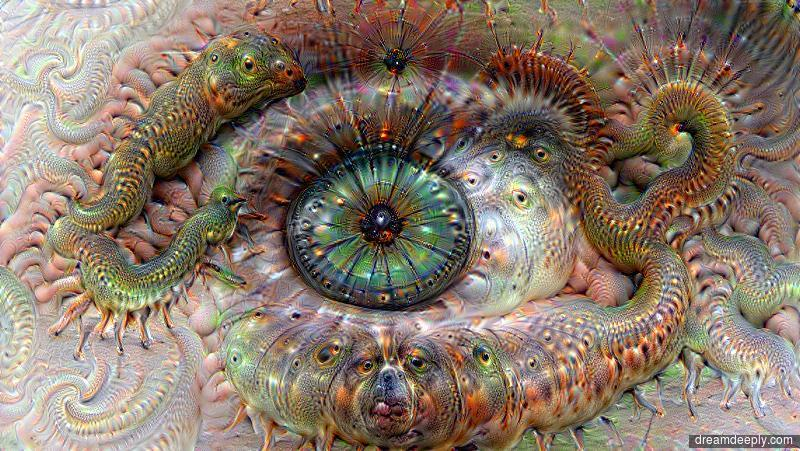
\includegraphics[scale=0.2]{images/title.jpg}}

\renewcommand{\vec}[1]{{\mathbf{#1}}}

\begin{document}

\begin{frame}
    \titlepage
\end{frame}

\frame {
    "Jede hinreichend fortgeschrittene Technologie ist von Magie nicht mehr zu unterscheiden."

    \begin{flushright}
    \textsl{Arthur C.\ Clarke}
    \end{flushright}
}

\frame{
    \frametitle{Überblick}
    \tableofcontents 
}

\section{Entwicklungen}

\frame {
    \frametitle{Entwicklungen: Was war}

    \begin{center}
    
\includegraphics[scale=0.23]{images/vista.jpg}

    \vfill

    \href{https://www.youtube.com/watch?v=-0kDcUEDfmY&feature=youtu.be&t=26s}{Video: Microsoft voice recoginition}
    \end{center}
}

\frame {
    \frametitle{Entwicklungen: Was ist}

    \begin{center}
    \only<1> { 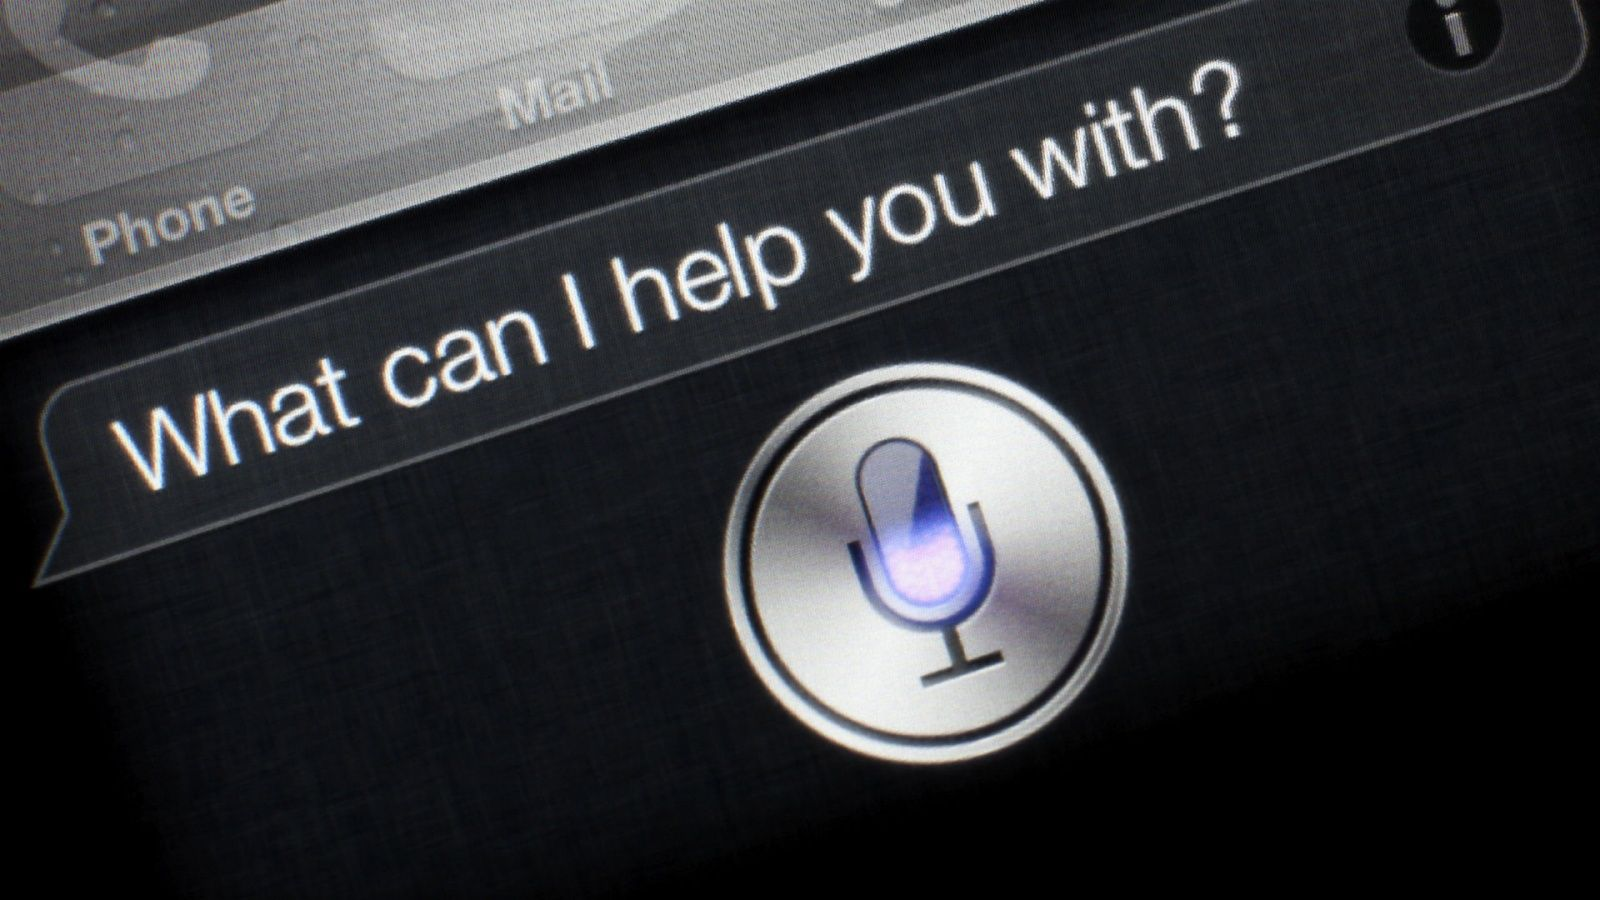
\includegraphics[scale=0.16]{images/siri.jpg} }
    \only<2> { 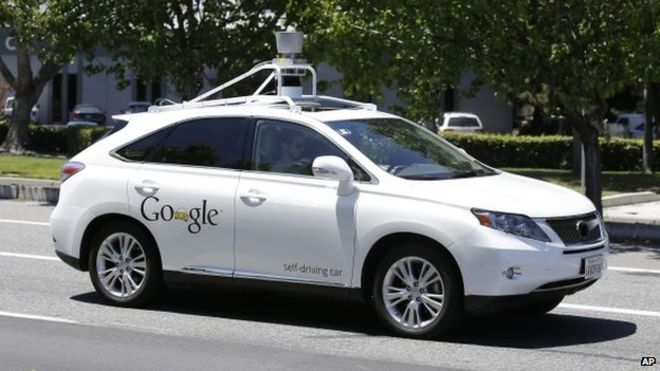
\includegraphics[scale=0.36]{images/googlecar.jpg} }
    \only<3> { 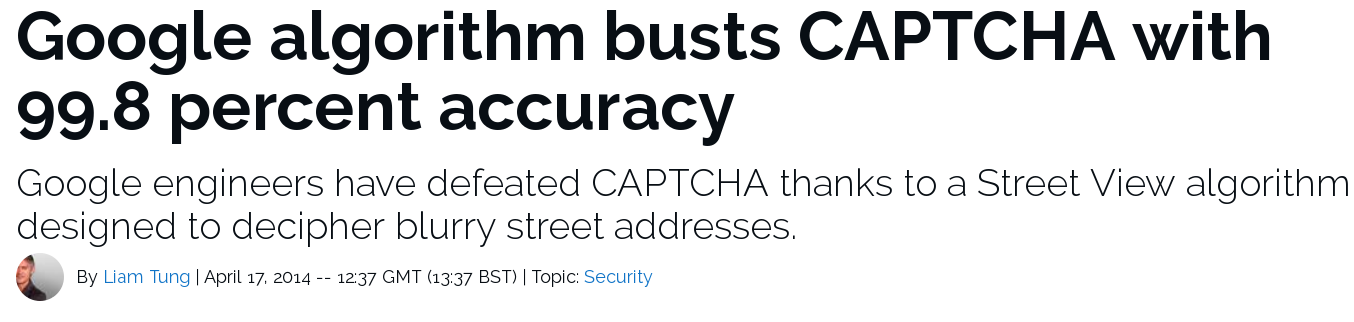
\includegraphics[scale=0.34]{images/captcha.png} }

    \vfill

    \only<1> { \href{https://www.youtube.com/watch?v=X9VCtPuBTBk&feature=youtu.be&t=10s}{Video: Siri} }
    \only<2> { \href{https://www.youtube.com/watch?v=csvt6JBAwBk&feature=youtu.be}{Video: Googles selbstfahrende Autos} }
    \only<3> { \href{http://www.zdnet.com/article/google-algorithm-busts-captcha-with-99-8-percent-accuracy/}{Google algorithm busts CAPTCHA} }
    \end{center}
}

\frame {
    \frametitle{Entwicklungen: Was war}

    \begin{center}
    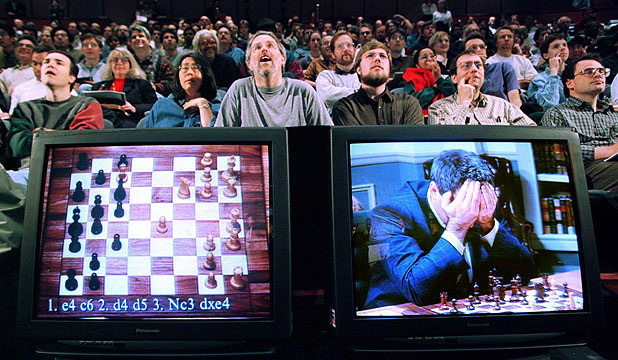
\includegraphics[scale=0.4]{images/deepblue.jpg}
    \end{center}
}

\frame {
    \frametitle{Entwicklungen: Was ist}

    \begin{center}
    
\includegraphics[scale=0.4]{images/alphago.png}
    \end{center}
}


\section{Erkennen von handgeschriebenen Ziffern}

\frame {
    \frametitle{Ehre wem Ehre gebührt}

    \begin{center}

    {\large \href{http://neuralnetworksanddeeplearning.com}{Neural Networks and Deep Learning}}

    \vfill

    von

    \vfill

     {\large \href{http://michaelnielsen.org/}{Michael Nielsen}}
    \end{center}

    \vfill
    \vfill
    \vfill

    \begin{flushright}
    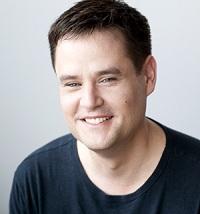
\includegraphics[scale=0.4]{images/nielsen.jpg}
    \end{flushright}
}

\frame {
    \frametitle{Erkennen von Ziffern}

    \begin{center}
    
\includegraphics[scale=0.2]{images/sequence.png}
    \end{center}

    \only<2->
    {
        \vfill
        Schwierigkeit für
        \begin{itemize}
        \item Menschen: extrem einfach
        \item (klassische) Algorithmen: extrem kompliziert
        \end{itemize}
    }
    \only<3>
    {
    \vfill
    Idee: \\
    Computer soll selbstständig lernen das Problem zu lösen
    }
}

\frame {
    \frametitle{Perceptron}

    \begin{center}
    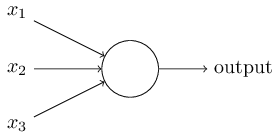
\includegraphics[scale=0.5]{images/perceptron.png}
    \end{center}

    \vfill

    \begin{itemize}
    \item mehrere binäre Eingänge $x_1,x_2,\dots$
    \item ein binärer Ausgang: output
    \item Gewichte $w_1,w_2,\dots$
    \item Schwellwert: threshold
    \end{itemize}

    \vfill

    \only<1>
    {
    \begin{equation}
    \nonumber
    \mathrm{output} = \begin{cases}
        0 \quad \mathrm{if} \quad \sum_j w_j x_j \le \mathrm{threshold} \\
        1 \quad \mathrm{if} \quad \sum_j w_j x_j >   \mathrm{threshold}
    \end{cases}
    \end{equation}
    }
    \only<2>
    {
    \begin{equation}
    \nonumber
    \mathrm{output} = \begin{cases}
        0 \quad \mathrm{if} \quad \vec w \cdot \vec x \le \mathrm{threshold} \\
        1 \quad \mathrm{if} \quad \vec w \cdot \vec x >   \mathrm{threshold}
    \end{cases}
    \end{equation}
    }
    \only<3>
    {
    \begin{equation}
    \nonumber
    \mathrm{output} = \begin{cases}
        0 \quad \mathrm{if} \quad \vec w \cdot \vec x +b \le 0 \\
        1 \quad \mathrm{if} \quad \vec w \cdot \vec x +b >   0
    \end{cases}
    \end{equation}
    }

}

\frame {
    \frametitle{Perceptron: Beispiel}

    \begin{center}
    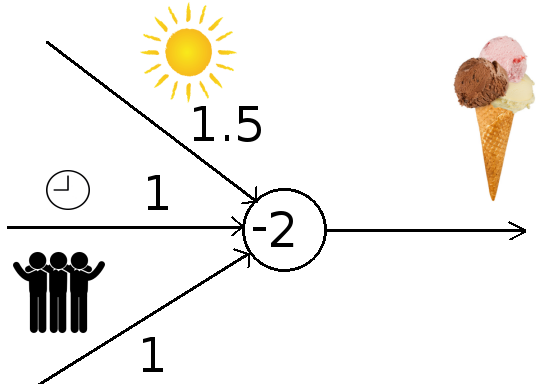
\includegraphics[scale=0.6]{images/perceptron_beispiel.png}
    \end{center}
}

\frame {
    \frametitle{Perceptrons sind universell}

    \begin{center}
    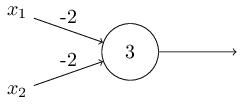
\includegraphics[scale=0.6]{images/perceptron_nand.png}
    \end{center}
}

\frame {
    \frametitle{Netzwerk aus Perceptronen}

    \begin{center}
    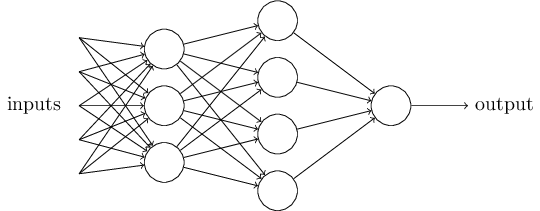
\includegraphics[scale=0.6]{images/perceptron_complex.png}
    \end{center}
}

\frame {
    \frametitle{Maschinelles lernen}

    Grundidee
    \begin{enumerate}
    \item Neuronales Netz erstellen
    \item Gewichte und Schwellwerte (bias) durch Training anpassen
    \end{enumerate}

    \vfill

    \begin{center}
    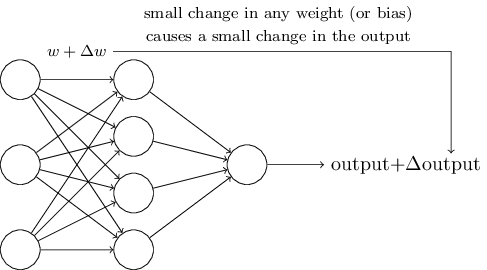
\includegraphics[scale=0.5]{images/delta.png}
    \end{center}
}

\frame {
    \frametitle{Sigmoids}

    \only<1>
    {
    Problem: \\
    Kleine Änderung der Gewichte/Schwellwerte kann komplettes Verhalten ändern
    }

    \only<2>
    {
    Lösung: Sigmoids
    \begin{itemize}
    \item kontinuierliche Eingangssignale $x_j \in [0,1]$
    \item Gewichte $w_j$, Schwellwert $b$
    \item Ausgabe: $\sigma(\vec w \cdot \vec x +b)$ mit $\sigma(z) = \frac{1}{1+\exp(-z)}$
    \end{itemize}

    \vfill

    \begin{equation}
    \nonumber
    \mathrm{output} = \frac{1}{1+\exp\left(-\vec w \cdot \vec x - b\right)}
    \end{equation}

    \vfill 
    \begin{center}
    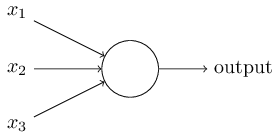
\includegraphics[scale=0.5]{images/perceptron.png} \quad 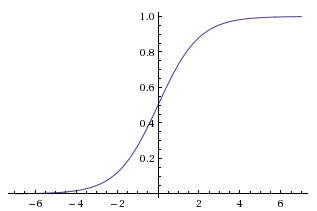
\includegraphics[scale=0.4]{images/fermi.png}
    \end{center}
    } 
}

\frame {
    \frametitle{Netzwerk}

    \begin{center}
    \only<1> { 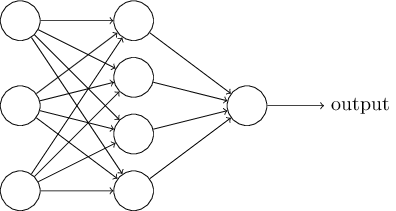
\includegraphics[scale=0.5]{images/network.png} }
    \only<2> { 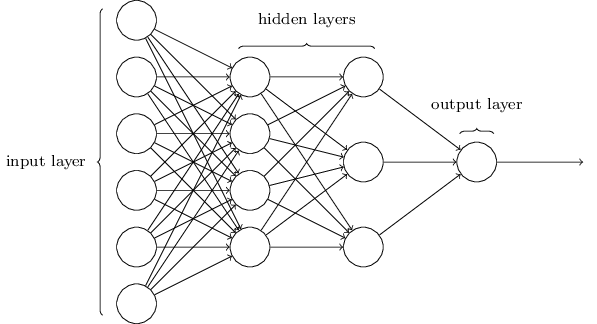
\includegraphics[scale=0.4]{images/network2.png} }
    \end{center}

    \vfill

    \begin{itemize}
    \item linke Schicht: input layer
    \item rechte Schicht: output layer
    \item mittlere Schichten: hidden layers
    \end{itemize}
}

\frame {
    \frametitle{Erkennen von Ziffern}

    \begin{itemize}
    \item Segmentation problem:
    \begin{center}
    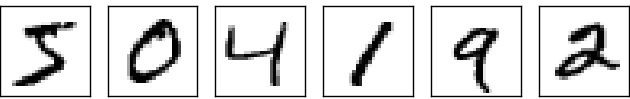
\includegraphics[scale=0.2]{images/sequence2.png}
    \end{center}

    gar nicht so leicht zu lösen...
    \item Erkennen der Ziffer

    Dieses Problem lösen wir. :)
    \end{itemize}
}

\frame {
    \frametitle{Netzwerk}

    \begin{center}
    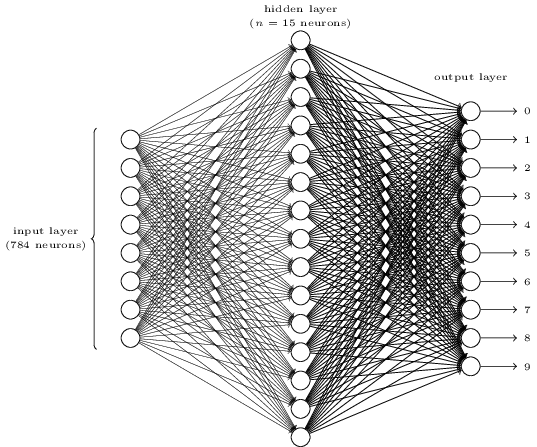
\includegraphics[scale=0.4]{images/network_recog.png}
    \end{center}

    \begin{itemize}
    \item $28^2$ Eingänge, $\vec x_\mathrm{in} \in \mathbb{R}^{784\times1}$
    \item $10$ Ausgänge, $\vec x_\mathrm{out} \in \mathbb{R}^{10\times1}$
    \item $f: \mathbb{R}^{784\times1} \to \mathbb{R}^{10\times1}$
    \end{itemize}
}

\frame {
    \frametitle{Trainingsdaten}

    MNIST: $60\,000+10\,000$ handgeschriebene Ziffern
    \begin{center}
    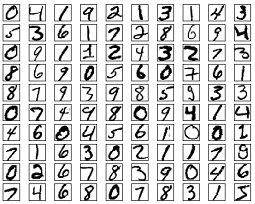
\includegraphics[scale=1]{images/mnist.png}
    \end{center}
}

\frame {
    \frametitle{Kostenfunktion}

    \only<1>   { $$C(\vec w_1,\dots,\vec w_n,b_1,\dots,b_n) = \frac{1}{2N} \sum_{\vec x \in \mathcal{T}} \left\| \, f(\vec x) - \vec a \, \right\|$$ }
    \only<2,3> { $$C(\vec p) = \frac{1}{2N} \sum_{\vec x \in \mathcal{T}} \left\| \, f(\vec x) - \vec a \, \right\|$$ }

    \only<1,2,3>
    {
    \begin{itemize}
    \item $\mathcal{T}$: Menge aller (Eingangs-)Trainingsdaten, $N=|\mathcal{T}|$
    \item $\vec a$: erwartetes (richtiges) Ergebnis für $\vec x$
    \item $f$: Wirkung des neuronalen Netzes
    \only<2> { \item $\vec p = (\vec w_1,\dots,\vec w_n,b_1,\dots,b_n)$ }
    \end{itemize}

    \only<3>
    {
    \vfill
    \hspace{10em} $\Rightarrow$ Minimiere $C(\vec p)$ !
    }
    }
}

\frame {
    \frametitle{Gradientenabstieg}

    $$\vec p_{j+1} = \vec p_j - \eta \, \nabla C(\vec p_j)$$

    \begin{center}
    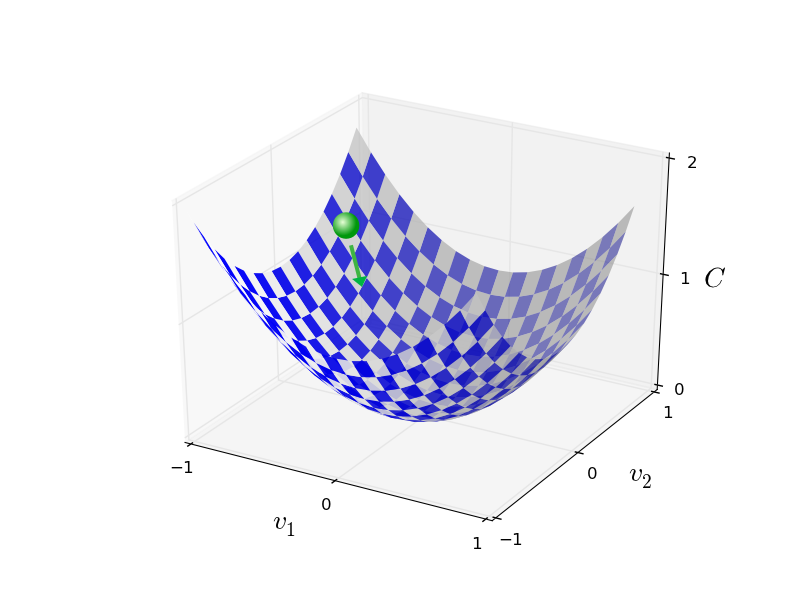
\includegraphics[scale=0.3]{images/gradient_descent.png}
    \end{center}
}

\frame {
    \frametitle{Demo}

    \begin{center}
    {\Huge Demo }

    \vfill

    online: \href{http://myselph.de/neuralNet.html}{http://myselph.de/neuralNet.html}
    \end{center}
}

\frame {
    \frametitle{Probleme}

    \begin{itemize}
    \item Lernprozess konvergiert gegen lokales (nicht globales!) Minimum
    \item Anpassung des Neuronalen Netzes auf Muster in den Trainingsdaten (z.B.\ hell/dunkel)
    \item Überanpassung (Auswendig lernen)
    \item Qualität der Traingsdaten (z.B.\ $1$)
    \item Daten müssen sinnvoll aufbereitet sein (z.B.\ Bild richtig gedreht und zugeschnitten)
    \item Netz muss für Problem geeignet sein
    \end{itemize}
}

\section{Ausblick}

\frame {
    \frametitle{Kopieren von Stilen}

    \begin{center}
    \only<1> { 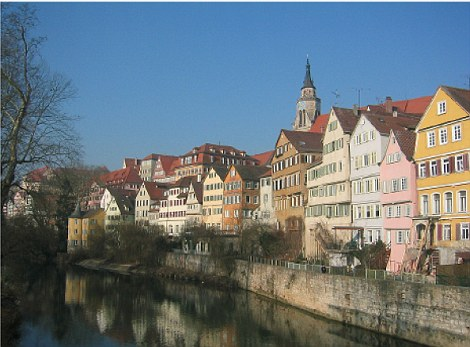
\includegraphics[scale=0.5]{images/orig.jpg} }
    \only<2> { 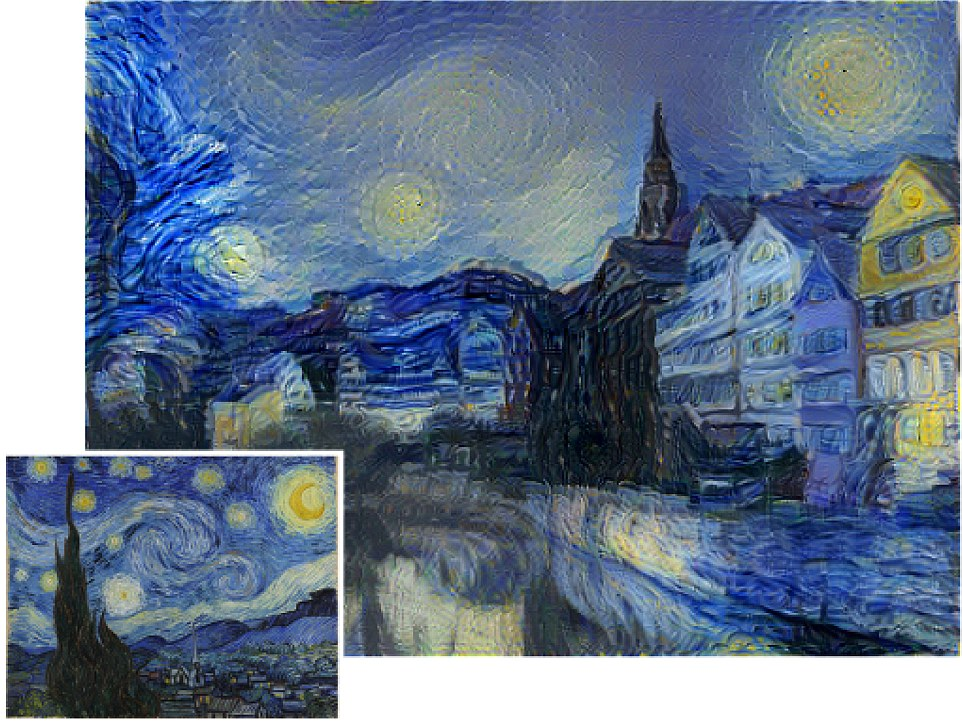
\includegraphics[scale=0.25]{images/van_gogh.jpg} }
    \only<3> { 
\includegraphics[scale=0.35]{images/odyseey.png}
    \vfill
    \href{https://vimeo.com/169187915}{Video: Picasso Odyssey}
    }
    \end{center}
}

\frame {
    \frametitle{Deep dreaming}

    \begin{center}
    \only<1> { 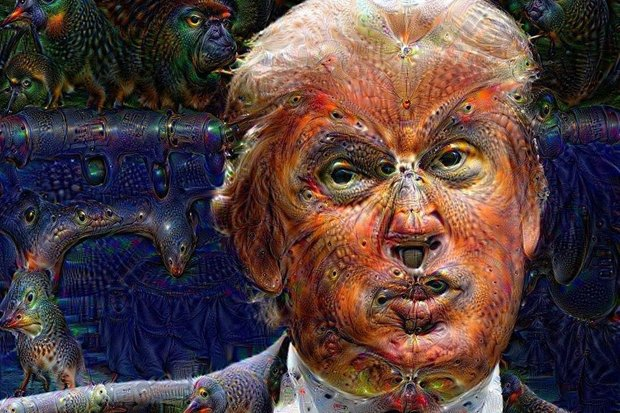
\includegraphics[scale=0.5]{images/trump.jpg} }
    \only<2> { 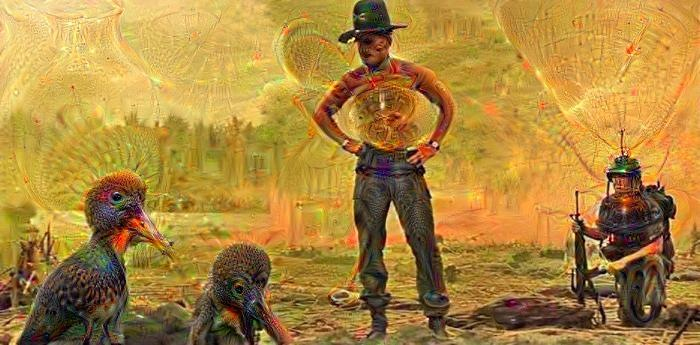
\includegraphics[scale=0.5]{images/apocalypse.jpg} }
    \only<3> { 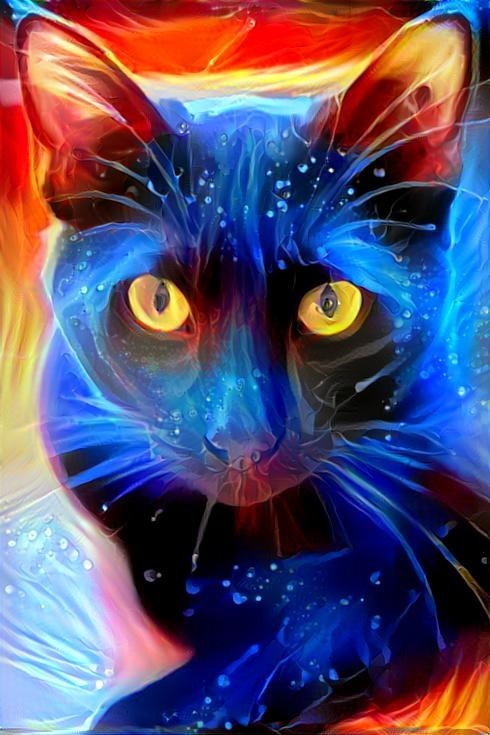
\includegraphics[scale=0.35]{images/cat.jpg} }

    \vfill
    \href{http://deepdreamgenerator.com/}{deepdreamgenerator.com}
    \end{center}
}

\frame {
    \frametitle{Vielen Dank für die Aufmerksamkeit :)}
    \begin{center}
    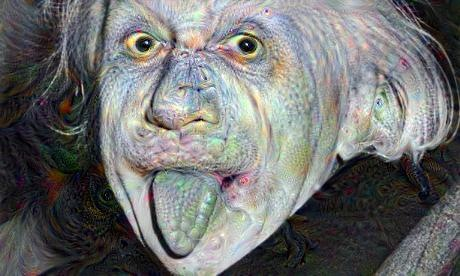
\includegraphics[scale=0.6]{images/einstein.jpg}
    \end{center}
}


\end{document}
